\documentclass{standalone}
\usepackage{tikz}
\usetikzlibrary{positioning}
\begin{document}
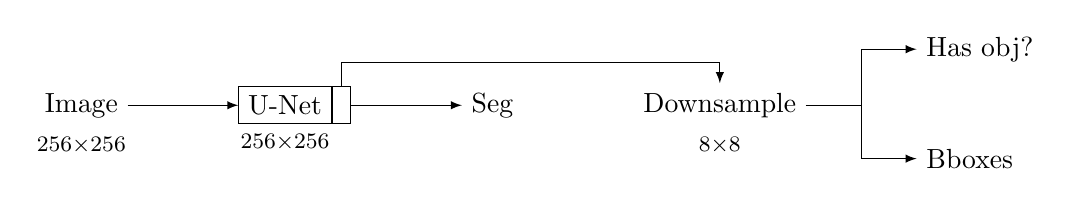
\begin{tikzpicture}[node distance=1ex and 4em]
\node (image) {Image};
\node [below=0pt of image, font=\footnotesize] {$256{\times}256$};
\node [draw, right=of image] (model) {U-Net};
\node [draw, right=0pt of model] (last) {\vphantom{U}};
\node [right=of last] (seg) {Seg};
\node [below=0pt of model, font=\footnotesize] {$256{\times}256$};
\node [right=of seg] (downsample) {Downsample};
\node [below=0pt of downsample, font=\footnotesize] {$8{\times}8$};
\node [above right=of downsample] (hasobj) {Has obj?};
\node [below right=of downsample] (bboxes) {Bboxes};

\draw[-latex] (image) -- (model);
\draw[-latex] (last) -- (seg);
\draw[-latex] (last.north) -- ++(0,2ex) -| (downsample.north);
\draw[-latex] (downsample.east) -- ++(2em,0) |- (hasobj);
\draw[-latex] (downsample.east) -- ++(2em,0) |- (bboxes);
\end{tikzpicture}
\end{document}
